
%% -*- coding:utf-8 -*-

\chapter{词汇功能语法}
%\chapter{Lexical Functional Grammar}
\label{Kapitel-LFG}


词汇功能语法(Lexical Functional Grammar,简称LFG)是上个世纪八十年代由Joan Bresnan和Ron Kaplan提出来的\citep{BK82a}。LFG是所谓的西海岸语言学的一个有机组成部分:不同于乔姆斯基任教的麻省理工学院,Joan Bresnan和Ron Kaplan在美国的西海岸工作(Joan Bresnan任教于斯坦福大学,而Ron Kaplan先后供职于帕罗奥图的施乐和加利福尼亚湾区Nuance的语言技术部门。)

\citet{BK82a}视心理语言学角度可行的可以替换转换的另一种分析方法。 For a discussion of
the requirements regarding the psycholinguistic plausibility of linguistics theories, see 
请参考第\ref{Abschnitt-Diskussion-Performanz}章以了解更多关于心理语言学角度下的语言学理论分析的可行性的讨论。 

想了解更多的基于LFG来分析德语的研究,可参阅\citew{Berman96a-u,Berman2003a} and \citew{Cook2001a}。

LFG有着设计良好的形式基础\citep{KB82a-u,Kaplan95a},正是基于这一点,LFG工程实践也开展得较早并取得成果
\citep*{FR83b,FR83a,Yasukawa1984a-u,BH86a-u,%
ED86a-u,% CHARON Parser
WA86a-u,%
Delmonte90a-u,% Italien
HHP91a-u,% Chinesisches kommerzielles System
Kohl92a-u,KGPRM92a-u,% ACORD project CHARON Generator
KM96a-u,%
Mayo97a-u,Mayo99a-u,%Konstanzer system
BS2005b-u,BS2005a-u,%SxLFG
Clement2009a-u,CK2001a-u% XLFG
}. 

The following is a list of languages with implemented LFG fragments, probably incomplete:
我们列举了一些已经实现出来的LFG语法片段:

\begin{itemize}
\item 阿拉伯语\il{Arabic} \citep{Attia2008a-u},
\item Arrernte\il{Arrernte} \citep*{Dras2012a-u},
\item 孟加拉语 \il{Bengali} \citep{SC97a-u},
%\item Chinese\il{Mandarin Chinese}
\item 丹麦语\il{Danish} \citep{Oersnes2002b-u,OW2003a-u,OW2004a-u},
\item 英语\il{English} \citep*{HHP91a-u,BDFK99a-u,RKKCMJ2002a-u,KM2007a-u},
\item 法语\il{French} \citep*{Zweigenbaum91a-u,Frank96b-u,FZ2002a-u,BDFK99a-u,CK2001a-u,BSL2005a-u,SdA2016a-u},
% Knueppel2001a-u
%
%
\item 格鲁吉亚语\il{Georgian} \citep{Meurer2009a-u},
\item 德语 \citep{Rohrer96a,Berman96a-u,KR97a-u,BDFK99a-u,Dipper2003a-u,RF2006a,Forst2006a-u,Frank2006a-u,FR2009a-u},
%\item Griechisch\il{Griechisch},
\item 匈牙利语\il{Hungarian} \citep{LRT2010a-u},
\item 印度尼西亚语\il{Indonesian} \citep*{AADMS2009a-u},
\item 意大利语\il{Italian} \citep*{Delmonte90a-u,Mayo99a-u,Quaglia2012a-u},
\item 爱尔兰语\il{Irish} \citep{Sulger2009a-u,Sulger2010a-u},
\item 日语\il{Japanese} \citep*{HHP91a-u,MO2003a-u,Umemoto2006a-u},
\item 韩语\il{Korean} \citep*{HHP91a-u},
\item 马达加斯加语\il{Malagasy} \citep*{Randriamasimanana2006a-u,DLM2006a-u},
\item 汉语普通话\il{Mandarin Chinese} \citep*{HHP91a-u,FK2007a-u},
\item Murrinh-Patha\il{Murrinh-Patha} \citep{SN2012a-u},
\item 挪威语\il{Norwegian} \citep*{DMR2005a},
\item 波兰语\il{Polish} \citep*{PP2012a-u},
\item 葡萄牙语\il{Portuguese} \citep{Alencar2004a-u,Alencar2013a-u},
\item 西班牙语\il{Spanish} \citep{Mayo99a-u},
\item 提格里尼亚语\il{Tigrinya} \citep{Kifle2012a-u},
\item 土耳其语\il{Turkish} \citep{CO2006a-u},
\item 匈牙利语\il{Hungarian} \citep*{LRT2010a-u,RLC2011a-u},
\item 乌尔都语/北印度语\il{Urdu}\il{Hindi} \citep*{BHKR2007a-u,BBS2008a-u},
\item 威尔士\il{Welsh} \citep{MS2005a-u}
and
\item 沃洛夫语\il{Wolof} \citep{Dione2012b-u,Dione2013a-u}.
\end{itemize}
上述语法中很多都是基于ParGram开发的\footnote{
  \url{http://pargram.b.uib.no/research-groups/}. 01.10.2015.
} \citep*{BKNS99a-ed,BDKMR02a-u}. 
除了上述语法,一个针对北梭托语\il{Northern Sotho}的语法也正在研发\citep{Faasz2010a-u}. 

Many of the LFG systems combine linguistically motivated grammars with a statistical
component.\is{statistics} Such a component can help to find preferred readings of a sentence first,
it can increase the efficiency of processing and make the complete processing robust (for instance
\citealp{KRKMVC2004a-u,RKKCMJ2002a-u}). Josef van Genabith's group in Dublin is working on the induction of
LFG grammars from corpora (\eg \citealp{JGCCR99a-u,DBCGW2005a-u,CBFDRCW2005a-u,CG2006a-u,GWG2007a-u,CBDRGW2008a-u,SG2009a-u}). 
很多LFG系统除了使用以语言学为准的语法,还使用统计模块\is{statistics}。
这样的模块可以帮助搜索一个句子最为倾向的解读分析。统计模块可以增强语言处理的效率,也可以增强系统鲁棒性(如\citealp{KRKMVC2004a-u,RKKCMJ2002a-u})。
Josef van Genabith在都柏林的团队目前正在研究如何从语料中自动约归出LFG语法。

\pagebreak
Some of the systems can be tested online:
很多系统都提供在线测试功能,如:
\begin{itemize}
\item \url{http://iness.uib.no/xle-web/xle-web}

% Statistik Dublin
\item \url{http://lfg-demo.computing.dcu.ie/lfgparser.html}
\item \url{http://www.xlfg.org/}
\end{itemize}




\section{关于表示形式的一般说明}

\label{Abschnitt-Format-LFG}

LFG假设多层表达。\footnote{
  本节中英语例句及其分析选自于\citet{Dalrymple2001a-u} and \citet{Dalrymple2006a}.
} 最重要的是c-结构\is{c"=structure}和f-结构\is{f"=structure}. 
c-结构是结构成分结构,其需要被一个具体的短语结构语法允准。
如果适合,这个短语结构语法使用\xbar~结构进行分析。
f-结构则意为功能结构。
功能结构包括的信息囊括了一个具体的结构成分中出现的谓词以及语法法能。
在不同的结构之间需要设立它们的映射关系。

\subsection{功能结构}

在LFG中, 诸如主语和宾语这样的语法功能发挥着非常重要的作用。
不同于大多数本书中讨论的其他理论,它们是LFG理论中的基本元素。
一个句子,如(\mex{1}a),可被赋予如(\mex{1}b)所示的功能结构:


\eal
\ex David devoured a sandwich.
\ex \lfgms{ pred & `DEVOUR\sliste{\lfgsubj, \lfgobj}'\\
         subj & \lfgms{ pred &  `DAVID' \\
                   }\\
         obj  & \lfgms{ spec & A\\
                     pred & `SANDWICH'\\
                   }\\
       }
\zl

\noindent
所有的产生语义的词汇项都贡献一个\textsc{pred}\isfeat{pred}特征及其取值。
被一个头词所管辖(此处管辖意为子类化)的语法功能为\textsc{pred}所规范\footnote{
在(\mex{0}b)中, 紧跟在\emph{devour}后面的\lfgsubj{}和\lfgobj{}即是整个结构中的\lfgsubj{}和\lfgobj{}。
出于紧凑表征的原因,这种同一关系并不在结构中进行显性表示。
}
这些功能被成为管辖语法功能(\emph{governable grammatical functions})\is{grammatical function!governable}。
表~\ref{Tabelle-GOV}罗列了一些管辖语法功能\citep{Dalrymple2006a}。
\begin{table}
\centering
\begin{tabular}[t]{@{}lp{26em}@{}} 
\lsptoprule
\textsc{subj}\isfeat{subj}: & 主语 \\ 
%
\textsc{obj}\isfeat{obj}: & 宾语\\ 
%
\textsc{comp}\isfeat{comp}: & 小句类型补足语或自足型(非谓词性)不定式补足语\\
\textsc{xcomp}\isfeat{xcomp}: & 非自足性(谓词性)补足语,经常为不定式,经常有一个外部的成分供职\is{control}其\textsc{subj}\\
\objtheta: & 第二宾语功能,经常配置一些特定的且语言相关的语法角色。在英语中其为且仅为\objtheme。\\ 
%
\obltheta: & 一组题元受限的需要显性语法标记的语法功能,如{\obl\downlett{GOAL}}或{\obl\downlett{AGENT}}。
             它们经常对应于c-结构中的介词短语。\\
\lspbottomrule
\end{tabular}
\caption{\label{Tabelle-GOV}管辖语法功能}
\end{table}\todostefan{\objtheta im Deutschen?}%
\pred 约定对应于GB理论中的题元格\is{theta-grid@$\theta$-grid}。
头词的配价\is{valence}信息也包含在\predv的约定信息中。

表\vref{Tabelle-NGOV}介绍了非管辖语法功能。
\begin{table}
\centering
\begin{tabular}[t]{@{}lp{26em}@{}} 
\lsptoprule
\textsc{adj}\isfeat{adj}: & 附属语 \\ 
%
\textsc{topic}\isfeat{topic}: & 语段的话题\\ 
%
\textsc{focus}\isfeat{focus}: & 语段的焦点\\
\lspbottomrule
\end{tabular}
\caption{\label{Tabelle-NGOV}非管辖语法功能}
\end{table}%
话题\is{topic|(}和焦点\is{focus|(}是信息结构(Information Structure)中的术语。
关于二者有一系列精确但相互之间并不完全相同的定义\citep[\page 253--254]{KruijffSteedman2003}。
宽泛地说来,一个语段的焦点是新信息之所在,而话题则是旧有的、已知的信息。
\citet[\page 97]{Bresnan2001a}使用如下的问句测试来区分话题与焦点。

\ea
\label{bsp-fronted-focus}
Q: What did you name your cat?\\
A: Rosie I named her. (\emph{Rosie} = \textsc{focus})
\z
\ea
\label{bsp-fronted-topic}
Q: What did you name your pets?\\
A: My dog, I named Harold. My cat, I named Rosie. (\emph{my dog}, \emph{my cat} = \textsc{topic})
\z
\is{topic|)}\is{focus|)}

\noindent
f-结构可以由功能描述(functional descriptions)来确立。
例如,我们可以通过下面的描述来确定一个功能结构$f$中的\textsc{tense}特征

\ea
($f$ \lfgtense)
\z

\noindent
可以在一个功能描述中去声明一个特征的具体取值。
下面的这个功能描述则进一步说明了在$ f$中,其\lfgtense{}特征取值为\lfgpast。

\ea
($f$ \lfgtense) = \lfgpast
\z

\noindent
有时候一个特征的值为另一个f-结构。
(\mex{1})中的表达式声明了$ f$的\subjf为f-结构$g$:

\ea
\label{ex-LFG-constraint}
($f$ \lfgsubj) = $g$
\z

\noindent
对应于(\mex{1}a)中的分析,我们可以得到(\mex{1}b)中的约束:
\eal
\ex David sneezed.
\ex
\begin{tabular}[t]{l}
($f$ \pred) = {\small `SNEEZE\arglist{\lfgsubj}'}\\
($f$ \lfgtense) = \lfgpast\\
($f$ \lfgsubj) = $g$\\
($g$ \pred) = {\small `DAVID'}
\end{tabular}
\zl

\noindent
(\mex{0}b)可描述了下述结构:
\ea
$f$: \lfgms{ pred  & {\small `SNEEZE\arglist{\lfgsubj}'}\\
             tense & \lfgpast\\
             subj  & $g$: \onems{ pred {\small `DAVID'} }\\
        }
\z

\noindent
需注意的是(\mex{-1}b)同样也可以描写许多其他的结构,这些结构可以包括一些扩展的特征。
在所有的这些包括了功能结构的全部新的结构中,我们仅仅关心那些极小结构(minimal structures)。

(\mex{1})展示了c-结构中的结点是如何和f-结构联系起来的:

\ea
%\ex David sneezed.
%\ex 
%% \begin{tabular}[t]{@{}ll@{}}
%% \begin{tabular}[t]{@{}cc@{}}
%% \multicolumn{2}{c}{\rnode{ip}{IP}}\\[2ex]
%% \rnode{b}{\rnode{np}{NP}}       & \rnode{i1}{I$'$}\\[2ex]
%% \rnode{n1}{N$'$}     & \rnode{vp}{VP}\\[2ex]     
%% \rnode{n}{N}         & \rnode{v1}{V$'$}\\[2ex]   
%% \rnode{David}{David} & \rnode{v}{V}\\[2ex]       
%%                     & \rnode{sneezed}{sneezed}\\
%% \end{tabular}
%% &
%% \lfgms{
%% pred & `SNEEZE\arglist{\lfgsubj}'\\
%% tense & PAST\\
%% subj  & \rnode{i}{\lfgms{ pred & `DAVID' \\
%%                       }}\\
%% }\\
%% \ltor[-15]{b}[175]{i}
%% \Aput*{$\phi$}
%% \end{tabular}
\tree{IP}{%
  \tree[b]{NP}{\tree{N$'$}{\tree{N}{\le{David}}}}
  \tree{I$'$}{\tree{VP}{\tree{V$'$}{\tree{V}{\le{sneezed}}}}}}%
\hspace*{4em}%
\raisebox{-2em}{\lfgms{
pred & {\small `SNEEZE\arglist{\lfgsubj}}'\\
tense & \lfgpast\\
subj  & \rnode{i}{\lfgms{ pred & {\small `DAVID'} \\
                      }}\\
}}\\
\ltor[-15]{b}[175]{i}
\Aput*{$\phi$}
\z
$\phi$指明NP结点与其相对应的f-结构之间的映射关系,在图中用一个标有$\phi$信息的箭头进行表示。

一个短语和它的中心词一直对应于同一个f-结构。

\ea
\begin{tabular}[t]{@{}c@{}}
\rnode{a}{\rnode{v1}{V$'$}}\\[2ex]
\rnode{b}{\rnode{v}{V}}\\[2ex]
\rnode{sneezed}{sneezed}\\
\end{tabular}
\hspace*{4em}
\rnode{d}{\raisebox{-2em}{\lfgms{ pred & {\small `SNEEZE\arglist{\lfgsubj}'}\\
                                  tense & \lfgpast}}}
\ncline{v1}{v}\ncline{v}{sneezed}%
\ltor{a}{d}
\Aput*{$\phi$}
\ltor{b}{d}
\z

\noindent
在英语的LFG语法中,\gbt所提出的CP/IP分析仍然被采用。
IP、I$'$和I(亦包括VP)被映射到同一个f-结构上。

\eal
\ex David is yawning.

\ex {\tree[a]{IP}{%
  \tree{NP}{\tree{N$'$}{%
    \tree{N}{\le{David}}}}
  \tree[b]{I$'$}{%
    \tree[c]{I}{\le{is}}
    \tree[d]{VP}{\tree[e]{V$'$}{\tree[f]{V}{\le{yawning}}}}}}}%
\hspace*{4em}%
{\rnode{o}{\raisebox{-2em}{\lfgms{ pred & {\small `YAWN\arglist{\lfgsubj}'}\\
                                   tense & \lfgpres\\
                                   subj  & \lfgms{ pred & {\small `DAVID'}}}}}}
\ltor{a}{o}
\ltor{b}{o}
\ltor[10]{c}{o}
\ltor{d}{o}
\ltor{e}{o}
\ltor{f}{o}
\zl



%% \subsubsection{Funktionale Eindeutigkeit ({\em Functional Uniqueness})}

%% {
%% {Funktionale Eindeutigkeit ({\em Functional Uniqueness})}

%% }

\noindent
f-结构需同时满足两个良形式条件:它们必须同时完备(complete)且一致(coherent)。我们将在后续章节中继续讨论这两个条件。

\subsection{完备性}

每一个中心词都增加一个关于\textsc{pred}特征取值的限制。完备性若满足,则需要\textsc{pred}值所约束的语法功能的元素全部实现。
在(\mex{1}b)中,\textsc{pred}所声明的\textsc{obj}在相应的f-结构中并未出现,因此(\mex{1}a)被LFG理论认为是不合语法的。

\eal
\ex[*]{David devoured.
}
\ex[]{
\lfgms{ pred & {\small `DEVOUR\sliste{\lfgsubj,\lfgobj}'}\\
         subj & \lfgms{ pred & {\small `DAVID'} \\
                   }\\
       }
}
\zl

\subsection{一致性}

\addlines
一致性条件要求在一个给定的f-结构中,所有的论元功能都必须局部地被同一个\textsc{pred}特征的取值所声明。
例(\mex{1}a)的不合语法性即由此而来:\textsc{comp}并没有作为论元出现在\emph{devour}的声明中。

\eal
\ex[*]{
David devoured a sandwich that Peter sleeps.%\\
%`David verschlang ein Sandwich, daß Peter schläft.'
}
\ex[]{
\lfgms{ pred & {\small `DEVOUR\sliste{\lfgsubj,\lfgobj}'}\\
         subj & [ \textsc{pred} {\small `DAVID'} ] \\
         obj  & \lfgms{ spec &  A\\
                     pred & {\small `SANDWICH'}\\
                   }\\
         comp & \lfgms{ pred & {\small `SLEEP\sliste{\lfgsubj}'}\\
                        subj & \lfgms{ pred & {\small `PETER'}\\
                                     }\\
                   } 
       }
}
\zl

\noindent
完备性与一致性限制共同确保了仅有且所有出现在\pred声明中的论元被实现出来。
这两条限制合在一起对应于\gbt中的题元准则\is{theta-criterion@Theta"=Criterion}(详见第\pageref{theta-Kriterium}页)。\footnote{
了解更多的关于LFG中的谓词论元结构与基于题元准则的深层结构之间的区别,可参阅\citew[\page xxvi--xxviii]{BK82a}。
} 


\subsection{c-结构与f-结构之间关系的限制}

为了得到f-结构,可以给c-结构中的符号\is{c"=structure|(}分配语法限制标注。
令`\up'\is{$\uparrow$}指示c-结构中的直接支配某结点的结点(即父结点)所对应的f-结构,
`$\downarrow$'\is{$\downarrow$}指示当前结点所对应的f-结构。
`\up~=~\down'是一个普遍被采用的限制标注。
这个限制声明了父结点的f-结构和当前结点的f-结构同一。

\ea
V$'$ $\to$ \begin{tabular}[t]{@{}r@{~=~}l@{}}
           \multicolumn{2}{@{}l@{}}{\hspaceThis{f-structure of the mother~}V}\\
           $\uparrow$ &  $\downarrow$\\ 
           父结点的f-结构 & 自身f-结构\\
           \end{tabular}
\z
`\up~=~\down'标注置于一个结构的中心词\is{head}之下。

在(\mex{0})中,
被经过标注的c-结构所允准的短语可做如下表示:
\ea
\talltree[a]{V$'$}{\le[b]{V}}%
\hspace*{3em}%
\rnode{d}{[\ ]}
\ltor{a}{d}
\ltor{b}{d}
\z

\noindent
(\mex{1})展示了一条带有一个宾语的V$'$规则:
\ea
\phraserule{V$'$}{
\rulenode{V\\* \up~=~\down}
\rulenode{NP\\*(\up\ \lfgobj) = \down}}
\z
%
``NP''对应的标注声明了其父结点所对应的f-结构中的\textsc{obj}(即mbox{(\up\ \lfgobj)}),其值为此``NP''所对应的f-结构,
亦即``NP''结点下方成分(\down)所对应的全部功能信息。
可视化展示见(\mex{1})中的图:
\ea
\talltree[a]{V$'$}{\le[b]{V} \le[c]{NP}}%
\hspace*{3em}%
\rnode{d}{\fd{\fdand{\feat{\lfgobj}{\rnode{e}{[\ ]}}}}}
\ltor{a}{d}
\ltor[20]{b}{d}
\ltor{c}[190]{e}
\z
在等式(\up\ \lfgobj) = \down{}中,箭头`\up'和`\down'对应于特征结构。
以(\ref{ex-LFG-constraint})为例,`\up'和`\down'分别代表了$f$和$g$。

(\mex{1})是一个不及物动词的例子,而(\mex{2})为对应的可视化展示:

\ea
\catlexentry{sneezed}{V}{(\up\ \pred) = {\small `SNEEZE\arglist{\lfgsubj}'}\\*
                     (\up\ \lfgtense) = \lfgpast}
\z

\ea
\tree{V}{\le{sneezed}}
\hspace*{4em}
\rnode{d}{\mbox{\lfgms{ pred & {\small `SNEEZE\arglist{\lfgsubj}'}\\
                        tense & \lfgpast}}}
\ltor{top}{d}
\z
\is{f"=structure|)}\is{c"=structure|)}\il{English|)}

\subsection{语义}
\label{lfg-semantics}
\label{glue-semantics}

依据\citet[\page 90--92]{Dalrymple2006a},胶粘语义(\emph{glue semantics})is{glue semantics|(}是LFG的一个主流语义分析方法
(\citealp*{DLS93a-u}; \citealp[Chapter~8]{Dalrymple2001a-u})。
另有一些基于Kamp's的篇章表示理论(discourse representation structures)\citep{KR93a}的分析方法\citep{FR83b,FR83a}。

In the following, glue semantics will be presented in more detail.
接下来我们将讨论胶粘语义的一些细节\footnote{
%The following section is a translation of the corresponding section in  \citew{Dalrymple2006a}.
下面的讨论对应于\citew{Dalrymple2006a}的相关章节。
}
在一个基于胶粘的方法中,我们假设f-结构是服务于语义解释的核心句法表征。
不同于\gbt,并不是一个论元在句法树中的位置参与语义的组合过程,而是诸如\lfgsubj和\lfgobj 之类的功能关系。 
胶粘语义假设f-结构中的每一个子结构都对应一个语义资源(semantic resource),不仅如此,整个结构的语义来自于子结构之和。
而语义的组合集成要遵循一定的规则,这些规则以线性逻辑\is{linear logic}的前提给出,在这种方法中,线性逻辑视为一种胶粘语言(glue language\is{glue language})。
语义的计算对应着通过逻辑推导出来的结论。

%\addlines[2]
这样的结论是通过逻辑前提推导而出的,这些前提来自于词也可能来自于一个句法构式(construction)本身。
而子部分语义如何进行组合成完整的语义则是通过一种基于资源(resource)的逻辑——线性逻辑——进行约束。
线性逻辑不同于经典逻辑,它不允许推导中出现不被使用的前提,也不允许一个前提被多次使用。
因此在线性逻辑中,前提是将要被使用的资源。
这直接对应于一个词在一个表达里的使用:词一次性服务于整个语义解释。
词既不能在语义解释中被略掉,也不可以在不同的部分多次贡献自己的力量。
句子\emph{Peter knocked twice.}的意义并不等同于\emph{Peter knocked}。
词\emph{twice}的语义必须被囊括到整个句子的完整语义中。
类似地,其句义也不同于\emph{Peter knocked twice twice.},因为词\emph{twice}的语义不可以被使用两次。

The syntactic structure for the sentence in 
(\mex{1}b)展示了例句(\mex{1}a)的句法及语义分析:
%Figure~\vref{c-f-sem-david-yawned}:
\eal
\ex David yawned.
\ex ~\\[-\baselineskip]
\hspace*{-2em}
{\ctree[ip]{IP}{%
  \tree[b]{NP}{\tree[n]{N}{\le{\em David}}}
  \tree[ii]{I$'$}{\tree[vp]{VP}{\tree[v]{V}{\le{\em yawned}}}}}}%
\hspace*{3em}%
{\fd{\rnode{s}{\fdand{\feat{\pred}{\small `YAWN\arglist{\subj}'}
           \feat{\subj}{\rnode{i}{\fdand{\feat{\pred}{\small `DAVID'}}}}}}}}%
\hspace*{2em}%
\mt{\relation{yawn}(\relation{david})}{\rnode{x}{~[\ ]}}
\ltor{ip}{s}
\Aput*{$\phi$}
\ltord[-10]{s}[220]{x}
\Bput*{$\sigma$}
\zl
%% \begin{figure}
%% \centerline{%
%% {\ctree[ip]{IP}{%
%%   \tree[b]{NP}{\tree[n]{N}{\le{David}}}
%%   \tree[ii]{I$'$}{\tree[vp]{VP}{\tree[v]{V}{\le{yawned}}}}}}%
%% \hspace*{3em}%
%% {\rnode{s}{\lfgms{ pred & {\small `YAWN\arglist{\lfgsubj}'}\\
%%                    subj & \rnode{i}{[ \textsc{pred} {\small `DAVID'} ]}}}}%
%% \hspace*{2em}%
%% \mt{\relation{yawn}(\relation{david})}{\rnode{x}{\;[\ ]}}
%% \ltor{ip}{s}
%% \Aput*{$\phi$}
%% \ltord[-10]{s}[220]{x}
%% \Bput*{$\sigma$}
%% }
%% \caption{c-structure, f-structure and semantics of \emph{David yawned.}}\label{c-f-sem-david-yawned}
%% \end{figure}%
% 
这一例句的语义结构与f-结构之间的关联通过关联函数$\sigma$(见虚线)进行表示。
这个语义表示从动词\emph{yawned}的词汇信息(见(\mex{1}))推导而得。

\ea
\mt{\lambda x. \relation{yawn}(x)}{(\up\ \lfgsubj)_\sigma\ \linimp\ \ups}
\z

\noindent 
这个公式被称为语义构建器(meaning constructor)\is{meaning constructor}。
其功能是将\emph{yawned}的语义——一个一元谓词$\lambda x. \relation{yawn}(x)$——和线性逻辑中的一个公式\is{\linimp}
\mbox{$(\up\ \lfgsubj)_\sigma\ \linimp\ \ups$}组合起来。
这里,连接词\linimp是线性逻辑中线性蕴涵的符号。
其意义为:一旦作为主语的语义资源$(\up\;\lfgsubj)_\sigma$可得,则必须产生一个新的语义资源$\up_\sigma$,
这个新的语义资源对应于整个句子的语义。 
不同于经典逻辑里的蕴涵算子,线性蕴涵必须消耗及产生语义资源:公式\mbox{$(\up\ \lfgsubj)_\sigma\ \linimp\ \ups$}
声明了如果发现了语义资源\mbox{$(\up\  \lfgsubj)_\sigma$},它将被消耗用以产生新的语义\ups。

进一步展开说来,假定一个像``David''这样的专有名词作为一个语义资源构成其语义结构。
以语段``David yawned''为例,``David''所对应的语义资源会被``yawned''所对应的语义资源消耗,
其原因在于``yawned''要求使用其\lfgsubj的语义资源以产生整个句子的语义资源。
这在直觉上很容易理解:任给一个句子,其中的动词需要其所有论元的语义,籍此方可理解整个句子。
that a verb in any given sentence requires the meaning of its arguments in order for the entire sentence to be understood.
  
``{David yawned}''的f-结构以及其中的``David''和``yawned''的语义构建器如(\mex{1})所示:

\eanoraggedright
 ~\\[-\baselineskip]
\fd{$y:$\rnode{s}{\fdand{\feat{\textsc{pred}}{\small `YAWN\arglist{\lfgsubj}'}
           \feat{\textsc{subj}}{$d:$\fdand{\feat{\textsc{pred}}{\small `DAVID'}}}}}}~\\[1em]
{$\begin{array}[t]{lr@{\;:\;}l}
\BF{David}&{\relation{david}}&{d_\sigma}\\*[1ex]
\BF{yawn}&{\lambda x. \relation{yawn}(x)}&{d_\sigma \linimp\ y_\sigma}
\end{array}$}
\z

\noindent 
标示为\BF{David}的语义构建器的左部为专有名词``David''的语义——\relation{david}。
而\BF{yawn}这一语义构建器的左部为相对应的不及物动词的语义——一个一元谓词$\lambda x. \relation{yawn}(x)$。

我们必须假定一些规则才能精确地确定(\mex{0})中语义构建器右部(即胶粘部分)和其左部(即语义部分)之间的关系。
对于像(\mex{0})中BF{David}这样的简单的、不包括逻辑蕴涵的语义构建器来说,
左部的语义等同与右侧的语义结构的语义。
而像\BF{yawn}这样的语义构建器,它们在左部里包含一个$\lambda$"-表达式,它们必须同其它的表达式通过
函数应用(functional application,详见\ref{sec-PSG-Semantik})。
而右部中的线性蕴涵也必须同步合并一个前提。
(\mex{1})展示了这样的一个合并过程。
在得到``{yawned}''和``{David}''之后,通过$\beta$-规约,
我们得到了句子``{David yawned}''的合理的语义分析结果——$\relation{yawn}(\relation{david})$ 

\ea
\label{ex:curryhoward}
$\begin{array}[t]{r@{\;:\;}l}
{x} & {f_\sigma}  \\
{P} & {f_\sigma\ \linimp\ g_\sigma} \\
\hline
{P(x)} & {g_\sigma}
\end{array}$
\z
规则的右部对应于演绎推理(modus ponens)\is{modus ponens}规则。
结合线性逻辑里的表达式与语义本身,我们可以得到(\mex{1})中的语义分析。
这个语义分析基于\citew[\page 92]{Dalrymple2006a}。
\begin{figure}[htb]
\ea
\label{ex:davidyawneddeduction}
\begin{tabular}[t]{r@{~:~}lp{18em}}
{\relation{david}} & $d_\sigma$ & 将语义\relation{david}分配给\lfgsubj的语义结构$d_\sigma$.\\[1em] 
$\lambda x. \relation{yawn}(x)$ & $d_\sigma \linimp\ y_\sigma$ & 如果我们在胶粘一侧找到了\lfgsubj的语义资源$d_\sigma$,
这个语义资源将被消耗,然后产生整个句子的语义资源$y_\sigma$。
而在语义一侧,我们将函数$\lambda x. \relation{yawn}(x)$应用到语义$d_\sigma$上。\\[1em]
\hline\multicolumn{3}{c}{}\\
$\relation{yawn}(\relation{david})$ & $y_\sigma$ &
我们构建了整个句子的语义资源$y_\sigma$,相对应地得到了整个句子的语义\relation{yawn}(\relation{david})。
\end{tabular}
\z
\vspace{-\baselineskip}
\end{figure}%
%
%\noindent 

\citep{Dalrymple99a-ed}讨论了针对量化(quantification)\is{quantification}、修饰和其它现象的胶粘语义分析。 
在针对语段中包含过多或过少语义资源的情形中,所讨论的这些方法会出现问题。
\citet{Asudeh04a-u}着重讨论了这些问题\is{glue semantics|)}。

\subsection{附属语}
\label{Abschnitt-LFG-Adjunkte}

附属语\is{adjuncts|(}并不被中心词选择。\textsc{adj}\isfeat{adj}这一语法功能是非管辖语法功能。
不同于语法功能只能实现一次的论元,一个句子可以包括多个附属语。
在一个f-结构中,\textsc{adj}特征的取值不能是一个单一的结构而是一个集合。
例如,例(\mex{1}a)的f-结构包括一个\textsc{adj}集合,这个集合中有两个元素:
``{yesterday}''和``{at noon}''。
\eal
\ex\label{ex-david-devoured-a-sandwich-at-noon-yesterday} David devoured a sandwich at noon yesterday.
\ex\label{fstruc-david-devoured-a-sandwich-at-noon-yesterday} 
\lfgms{ pred & `DEVOUR\sliste{\lfgsubj,\lfgobj}'\\
         subj & \lfgms{ pred &  `DAVID' \\
                      }\\
         obj  & \lfgms{ spec & A\\
                        pred & `SANDWICH'\\
                      }\\
         adj & \menge{ \lfgms{ pred & `YESTERDAY' },
                        \lfgms{ \pred & `AT\arglist{\lfgobj}'\\
                                obj   & \lfgms{ pred & `NOON' }\\
                              } }\\
}
\zl
%
针对附属语的c-结构的标注要求附属语是其父结点的\textsc{adj}集合的一部分:
\ea
\phraserule{V$'$}{
\rulenode{V$'$\\* \up~=~\down}
\rulenode{PP\\*\hbox {$\downarrow$\kern .2em} $\in$ (\up\ \adj)}}
\z
将附属语表示为一个集合不足以表示包括域(scope)信息的附属语(如页\pageref{bsp-absichtlich-nicht-anal}中的例句(\ref{bsp-absichtlich-nicht-anal})中所涉及的否定)。
为了确定域关系,我们必须参照附属语的在句子中的先后顺序,这就设计了c-结构信息。
想了解更多的关于序列化的限制,可以参考\citew{ZK95b}.\is{adjunct|)}。

\section{被动}
\label{Abschnitt-LFG-Passiv}

%Banksy: "If you don't own a train company then you go and paint on one instead."
% Bindung in ein Kompositum hinein, aber sehr merkwürdig.
% en.wikipedia.org/wiki/Banksy 20.01.2013

\mbox{}\citet{BM95a}\is{passive|(}\is{morphology|(}讨论认为我们可以视词为构造句法结构的原子成分(词汇完整性(lexical integrity)\is{lexical integrity}\ootnote{
 进一步了解词汇完整性,可参阅\citew[\page 84]{Anderson92a-u}。
})。

句法规则无法创造新的词,也无法引用词的内部结构信息。每一个终结结点(即树上上每一个叶子结点)均为词。
由此我们可以根据词汇完整性否定一些基于GB的分析,如\citet{Pollock89a-u}提出的针对法语例句(\mex{1})的分析(见表\vref{add-Pollock},该表选择\citealp[\page 617]{Kuhn2007a}):

% Felix sagt: So ist es richtig. Weicht von Jonas ab.
\ea
\gll Marie ne parlerait pas \\
     Marie \textsc{neg} speak.\textsc{cond.3sg} \textsc{neg}\\
\glt `Marie would not speak.'
\z
%
在Pollock的分析中,不同的词素在树中的不同位置,而且它们只有在移位之后才进行组合。

\begin{figure}
\centerline{%
\begin{forest}
for tree={parent anchor=south, child anchor=north,align=center,base=bottom}
[AgrP
	[Spec-AgrP,name=specagr]
	[Agr$'$
		[Agr
			[\textit{-ait},name=ait]]
		[NegP
			[Spec-NegP
				[\textit{pas},name=pas]]
			[Neg$'$
				[Neg
					[\textit{ne},name=ne]]
				[TP
					[Spec-TP]
					[T$'$
						[T
							[\textit{-er-},name=er]]
						[VP
							[Spec-VP
								[\textit{Marie},name=marie]]
							[V$'$
								[V
									[\textit{parl-},name=parl]]]]]]]]]]
\begin{pgfinterruptboundingbox}% otherwise the picture gets larger due to the control points
\draw[->,dotted] (parl.south west) .. controls +(225:1cm) and +(south:0.4cm) .. (er.south);
\draw[->,dotted] (er.south west) .. controls +(left:1cm) and +(south:0.4cm) .. (ne.south);
\draw[->,dotted] (ne.south west) .. controls +(left:1cm) and +(south:0.4cm) .. (ait.south);
\draw[->,dotted] (marie.-90) .. controls +(225:6cm) and +(250:3cm) .. (specagr.-90);
\end{pgfinterruptboundingbox}
\end{forest}
}\is{category!functional!Neg}\is{category!functional!T}\is{category!functional!Agr}
\caption{\label{abb-Pollock} Pollock给出的针对\emph{Marie ne parlerait pas} `Marie would not
  speak.'的分析,具体分析选自\citet[\page 617]{Kuhn2007a}}
\end{figure}%
除了GB和最简方案之外,本书中讨论的所有理论均接受词汇完整性这一假设。
尽管如此,形式上来说,词汇完整性并不是必须满足的性质,像CG、GPSG、HPSG、CxG、DG和TAG的形式理论均允许将词素和复杂句法结构联系起来。
据我所知,目前还没有人提出过这种类型的分析。

%\subsection{Passiv als lexikalischer Prozeß}

Bresnan注意到,和被动式的动词一样,也有被动式的形容词,这些形容词也有一致的形态异质性
(citealp[\page 21]{Bresnan82a}; \citealp[\page 31]{Bresnan2001a})。
(\mex{1})罗列了一些例子:

\eal
\label{ex-well-written}
\ex a well-written novel (write -- written)
\ex a recently given talk (give -- given)
\ex my broken heart (break -- broken)
\ex an uninhabited island (inhabit -- inhabited)
\ex split wood (split -- split)
\zl
\il{English|)}

\noindent
如果我们假定词汇完整性,那么我们必须在词典里去推导形容词。
如果动词性的被动的生成不是词汇处理过程,而是一个短语结构,那么形式的同一性仍然得不到解释。\is{morphology}\todostefan{wieso?}

在LFG中,语法功能\is{grammatical function}是基础要素,换句话说它们不是从句法树中的位置推导出来(如Subject = SpecIP)。
词(经过了完整曲折变化的词)决定了它的论元的语法功能。此外,语法功能还存在一个层级机构。
在分词形成的过程中,层级最高的动词性论元被抑制。
层级第二高的论元向上移动,进而会被实现为\textsc{subject}而不是\textsc{object}。
早期的工作明确地提出了上述分析方法\citep[\page 8]{Bresnan82a}:
\ea
被动规则:\\
\begin{tabular}{@{}l@{~$\mapsto$~}l@{}}
(\lfgsubj) & $\varnothing$/(\obl)\\
(\lfgobj)  & (\lfgsubj)
\end{tabular}
\z
第一条规则规定:主语要么实现为空($\varnothing$),要么实现为一个带语法标记的元素(如英语里的由``{by}''来引导的介词短语)。
第二条规则规定:如果存在宾格形式的宾语,则其实现为主语。

在后来的研究中,语法功能的分配逐渐为词汇映射理论(Lexical Mapping Theory)\is{Lexical Mapping Theory (LMT)|(}\is{linking|(}\label{page-LMT}所替代\LATER{\citep{Levin87a}}\citep{BresnanK89a-u}。 
按照假定,题元角色\is{semantic role|(}会按照一个普遍语法意义下的层级结构进行排序(\citealp{BresnanK89a-u}; \citealp[\page
307]{Bresnan2001a}): 施事\is{agent} $>$ 受益者\is{beneficiary} $>$ 感知者/目标\is{experiencer}\is{goal} $>$ 工具\is{instrument} $>$ 受事/主题\is{patient}\is{theme} $>$ 位置格。
在相应的被称之为a-结构\is{a"=structure}的表示体系中,受事类型会被标记为不受限([$-$r])。
第二受事类型的角色会被标记为宾格的([+o]),而所有的其它角色都会被标记为非宾格的([$-$o])。
对于德语及物动词``{schlagen}''(击打)而言,我们有如下分析:
\ea
\begin{tabular}[t]{@{}llll@{}}
           &          & 施事 & 受事 \\
a-结构 & \emph{schlagen} & $\langle$ x & y~~ $\rangle$\\
           &          & \hspaceThis{$\langle$}[$-$o]       & [$-$r] \\
\end{tabular}
\z

\noindent
%\addlines
从a-结构到f-结构的映射要收到如下限制:
\eal\label{lmt}
\ex
\begin{sloppypar}
   主语-映射-原则:\is{principle!Subject"=Mapping} 标记为[$-$o]的最优先的角色被映射为\lfgsubj,如果它是a-结构中的初始成分。
   否则,标记为[$-$r]的角色被映射为\lfgsubj。
\end{sloppypar}
\ex 论元角色与语法功能之间的对应关系如下表所示。未声明o与r取值的被认为是`+':

\begin{tabular}[t]{@{}lll@{}}
         & [$-$r] & [$+$r]\\
{}[$-$o] & \lfgsubj  & \obltheta\\
{}[$+$o] & \lfgobj   & \objtheta\\
\end{tabular}
\ex 功能-论元二元唯一性:每一个a-结构中的角色都必须关联到一个且仅此一个功能,反之亦然。
\zl
对于(\mex{-1})中的论元结构,原则 (\mex{0}a)确保了施事x关联到语法功能\lfgsubj。
(\mex{0}b)增加了一个o-特征,且值为`+',所以受事y关联到了\lfgobj :
\ea
\begin{tabular}[t]{@{}llll@{}}
           &          & 施事 & 受事\\
a-结构 & \emph{schlagen} & $\langle$ x & y~~ $\rangle$\\
           &          & \hspaceThis{$\langle$}[$-$o]    & [$-$r] \\\cline{3-4}
           &          & \hspaceThis{$\langle$}\lfgsubj       & \lfgobj
\end{tabular}
\z

\noindent
在被动中,最突出的角色被抑制了,只有[$-$r]标记的受事被保留下来。
按照(\ref{lmt}a),这个角色将要被映射为主语。
\ea
\begin{tabular}[t]{@{}llll@{}}
           &          & 施事 & 受事\\
a-结构 & \emph{schlagen}  & $\langle$ x & y~~ $\rangle$\\
           &          & \hspaceThis{$\langle$}[$-$o]    & [$-$r] \\\cline{3-4}
           &          & \hspaceThis{$\langle$}$\varnothing$       & \lfgsubj
\end{tabular}
\z

\noindent
和及物动词的宾语不同,像``{helfen}''(帮助)的宾语会被标记为[+o] \citep{Berman99a}。
因为格(与事)链接到语义角色上,因而宾语的词汇格\is{case!lexical}在a-结构中给出\citep*[\page 465]{ZMT85a}。
相关的语义角色必须影射到语法功能\objtheta上。
\ea
\begin{tabular}[t]{@{}llll@{}}
           &          & 施事 & 受益者\is{beneficiary}\\
a-结构 & \emph{helfen} & $\langle$ x & y~~ $\rangle$\\
           &          & \hspaceThis{$\langle$}[$-$o]    & [$+$o]/DAT \\\cline{3-4}
           &          & \hspaceThis{$\langle$}\lfgsubj       & \objtheta
\end{tabular}
\z
被动将会缠身下述结果:
\ea
\begin{tabular}[t]{@{}llll@{}}
           &          & 施事 & 受益者\is{beneficiary}\\
a-结构 & \emph{helfen} & $\langle$ x & y~~ $\rangle$\\
           &          & \hspaceThis{$\langle$}[$-$o]    & [$+$o]/DAT \\\cline{3-4}
           &          & \hspaceThis{$\langle$}$\varnothing$       & \objtheta
\end{tabular}
\z
因为既没有[$-$o]类型论元,也没有[$-$r]类型论元,没有论元能够链接到主语上。
这导致了非人称被动式中的论元与语法功能的结合。

这些影射原则乍看很复杂,但它们在分析相关的语言现象时发挥了很大的作用,如非宾格结构\is{verb!unaccusative}\citep{BZ90a}。
关于被动的分析,我们现在可以下这样的结论:被动抑制了层级最高的[$-$o]角色。
并没有什么必要在被动规则中提及最终的宾语。
%
\is{Lexical Mapping Theory (LMT)|)}\is{linking|)}\is{passive|)}\is{semantic role|)}

\section{动词位置}
\label{Abschnitt-Verbstellung-LFG}

关于德语中的动词位置\is{verb position}有两种可能的分析。
\begin{sloppypar}
\begin{itemize}
\item 在动词后置位置又一个语迹(参见GB\indexgb) (详见\citealp{Choi99a-u}, \citealp[Section~2.1.4]{Berman96a-u}) 
\item 所谓的中心词的扩展域(详见\citealp{Berman2003a})
\end{itemize}
\end{sloppypar}

\noindent
在中心词的扩展域的分析中,动词只不过是从动词短语中省略掉了。下面的VP规则的基本变种很常见\footnote{
\citet[\page 110]{Bresnan2001a}和\citet[Section~2.2]{Dalrymple2006a}中讨论了在规则右部出现一个可选组成成分的规则。
}
\ea
\label{Regel-LFG-VP-alles-optional}
VP $\to$ (NP) (NP) (NP) (V)
\z
动词短语的所有组成部分都是可选的,注意括号表示可以出现也可以不出现。
和GB的分析一致,动词在动词前置的小句中属于C范畴,而并不假设范畴I存在投射(\citealp{Haider93a,Haider95b-u,Haider97a}; \citealp[Section~IV.3]{Sternefeld2006a-u}),
这是出于对语言事实的考量\citep[Section~3.2.2]{Berman2003a}。动词会从C范畴位置提供f-结构信息。
图~\vref{Abb-Verbstellung-LFG}是\citet[\page 41]{Berman2003a}提出的简化分析。\todostefan{do all LFG figures without PS tricks}
 
\begin{figure}
\centerline{%
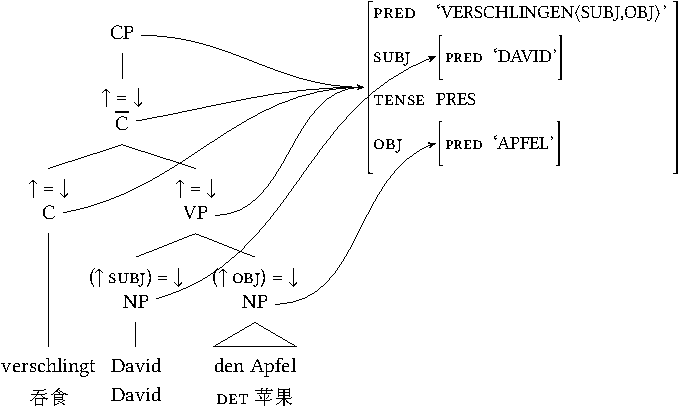
\includegraphics{Figures/verschlingt-david-den-apfel-lfg-lsp-crop}
}
\caption{\label{Abb-Verbstellung-LFG}遵循\citet[\page 41]{Berman2003a}的动词位置分析}
\end{figure}%

{\interfootnotelinepenalty=10%
\noindent
在了解了第\ref{Kapitel-PSG}章和第\ref{Kapitel-GPSG}章的短语结构规则后,允许动词短语确实动词看起来很不自然。
然而这对于LFG来说并不是一个问题,因为分析一个给定的句子,我们只需要保证所有必须要的成分(也只有这些成分)都出现。 
完备性\is{completeness}和一致性\is{coherence}的限制保证了这一点。究竟信息来自何方并不重要。
在图\ref{Abb-Verbstellung-LFG}中,动词信息并不来自于动词短语,而是C结点。
C$'$被下面的一个特殊规则所允准:
\ea
\phraserule{C$'$}{
\rulenode{C\\* \up~=~\down}
\rulenode{VP\\*\up~=~\down}}
\z
在LFG规则中,通常来说只有中心词这一个元素标记`\up~=~\down'。在(\mex{0})中,有两个这样的元素,这也是为什么二者同时为其夫结点的f-结构提供信息的原因。
动词的中心词域被C扩展了。\lfgsubj和\lfgobj 的信息来自于动词短语,而\pred信息则来自于C。
\is{head domain!extended|)}\is{verb"=final language}

\section{局部语序重列}
\label{Abschnitt-LFG-Umstellung}

在前人的工作中已经讨论过两种\is{constituent order}处理局部语序重列的方法\footnote{%
  \citet[\page 20--21]{Kaplan95a}讨论了如何在LFG中设计一个基于ID/LP\is{ID/LP grammar}形式的语法。
  而GPSG类型的组成成分顺序尚未在LFG框架中得以解决。%
}
\begin{itemize}
\item 像GB\indexgb一样在基本布局中移动论元(详见\citealp{Choi99a-u})
\item 直接在短语规则中允准(详见Berman \citeyear[Section~2.1.3.1]{Berman96a-u}; \citeyear{Berman2003a})
\end{itemize}

\noindent
如果我们假设语迹在给定结构的语义解释中是发挥作用的,则第一种分析和基于移动的GB分析有着一样的问题。
在\ref{sec-GB-lokale-Umstellung}中我们已经讨论过这些问题了。

接下来,我讨论\citet[Section~2.1.3]{Berman96a-u}提出的分析,在某种意义上来说我简化了表示。
动词论元的格和语法功能由词典所决定\citep[\page 22]{Berman96a-u}。
(\mex{1})展示了德语动词``\emph{verschlingen}''(吞食)的词汇项信息:\footnote{%
  德语的四个格可以用两个二元特征——{\small GOV}和{\small OBL}——进行表示\citep[\page 22]{Berman96a-u}。
  主格的{\small GOV}为$-$,而{\small OBL}为$-$;宾格的{\small GOV}为$+$,而{\small OBL}为$-$。
  这种类型的表示法使得我们可以仅仅通过部分信息来描述一个格。
  如果我们没有声明{\small GOV}的值,则一个{\small OBL}为$-$的格描述既和主格也和宾格兼容。
  因为下面的讨论并没有使用到这种局部声明的好处,我接下来并没有使用特征分解而是直接使用格信息。
}$^,$\footnote{%
  作为一种替代性分析,也可以从格中推导出一个名词短语的语法功能(\citealp[\page 37]{Berman2003a}提出的德语分析;\citealp[\page 187, \page 201]{Bresnan2001a}提出的德语和俄语分析\il{Russian})

\ea
\label{Kasus-Implikation-Berman}
\upshape      (\downsp \case) = \mdacc{} $\Rightarrow$ (\upsp \lfgobj) = \down{}
\z

\noindent
  \citet[Section~2.1]{Karttunen89a-u}在分析芬兰语的时候,基于范畴语法\indexcxg的框架提出了类似的分析。
  因为格并不总是非常可靠地与语法功能耦合在一起,因此类似的分析并非完全没有问题。
  在德语中,和时间宾格(ii.a)一样,有一些动词会有两个宾格宾语(ii.b--c)和谓词性宾格(ii.d)。

\eal
\ex 
\gll Er arbeitete den ganzen Tag.\\
	 he worked the.\acc{} whole.\acc{} day\\
\ex 
\gll Er lehrte ihn den Ententanz.\\
	 he taught him.\acc{} the.\acc{} duck.dance\\
\ex 
\gll Das kostet ihn einen Taler.\\
	 that costs him.\acc{} a.\acc{} taler\\
\ex 
\gll Sie nannte ihn einen Lügner.\\
	 she called him.\acc{} a.\acc{} liar\\
\zl
所有的这些宾格都可以出现在长距离依赖关系中(见\ref{Abschnitt-NLA-LFG}):

\ea
\gll Wen glaubst du, dass ich getroffen habe.\\
	 who believe you that I met have\\
\glt `Who do you think I met?'
\z

\noindent
``{wen}''并不是``glauben''的宾语,因此并不在``glauben''的f-结构中。
One would have to reformulate the implication in
(i) as a disjunction of all possible grammatical functions of the accusative and in addition account for the fact that accusatives can come from a more deeply embedded f"=structure.
}
\ea
\label{le-verschlingen}
\catlexentry{verschlingt}{V}{(\up\ \pred) = {\small `VERSCHLINGEN\arglist{\lfgsubj, \lfgobj}'}\\*
                             (\up\ \lfgsubj{} {\small AGR CAS}) = NOM\\*
                             (\up\ \lfgobj{} {\small AGR CAS}) = ACC\\*
                             (\up\ \lfgtense) = \small PRES}
\z

%\addlines
\largerpage
\noindent
Berman提出一种分析,在他的分析里,动词并不会和它的轮元及附属语同时结合,就像GPSG\indexgpsg里分析的那样。
她的分析走向另一个极端,她假设动词并不是和附属语或者轮元结合,而是直接形成动词短语。
相关的规则如(\mex{1}):所示:
\ea
\label{LFG-v-vp}
\phraserule{VP}{
\rulenode{(V)\\* \up~=~\down}}
\z
乍一看来,这种分析非常奇怪,显然一个像``devour''一样的动词,它自身的分布与它和它轮元加和之后的分布是并不相同的。
但是,我们应当回想一下保留下来的针对f-结构一致性与完备性的限制,它们仍然起作用,进而这个理论仍然不会做出错误的(针对语言现象的)预测。
}% footnote breaks

因为动词可以出现在初始位置,它在(\mex{0})规则里被标记为可选(见\ref{Abschnitt-Verbstellung-LFG})。

下面的规则可以用以进一步组合动词和它的主语或者宾语。
\ea
\label{lfg-vp-regel}
\phraserule{VP}{
\rulenode{NP\\* (\upsp \lfgsubj|\lfgobj|\objtheta) = \down}
\rulenode{VP\\* \up~=~\down}}
\z
这里的`|'\is{$\vert$}表示析取(disjunction\is{disjunction}),也就是说,NP既可以是相应f-结构的主语也可以是宾语。, that is, the NP can either be the subject or the object of the superordinate f"=structure. Since VP occurs both on the left
因为VP既出现在(\mex{0})中所示规则的左边也出现在其右边,它可以多次进行应用。
而这个规则并不完整。例如,我们还必须解释介词型宾语、小句型论元、形容词性论元和附属语。
参见第\pageref{fn-zp}页的脚注\ref{fn-zp}。

\largerpage
图\vref{Abb-SOV-LFG}展示了(\mex{1}a)的分析。 
\eal
\ex 
\gll {}[dass] David den Apfel verschlingt\\
      \spacebr{}that David the apple devours\\
\glt `that David is devouring the apple'
\ex 
\gll {}[dass] den Apfel David verschlingt\\
     \spacebr{}that the apple David devours\\
\zl
\begin{figure}
\centerline{%
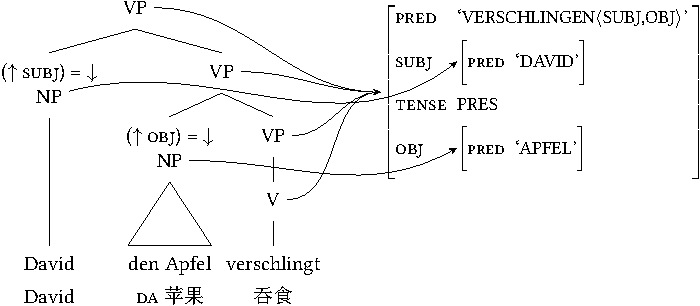
\includegraphics{Figures/david-den-apfel-verschlingt-lfg-lsp-crop}
}
\caption{\label{Abb-SOV-LFG}参考\citet{Berman96a-u}的针对SOV语序的分析}
\end{figure}%
(\mex{0}b)的分析见图\vref{Abb-OSV-LFG}。
\begin{figure}
\centerline{%
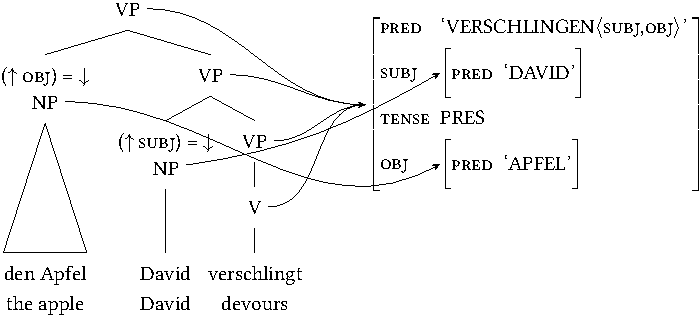
\includegraphics{Figures/den-apfel-david-verschlingt-lfg-lsp-crop}
}
\caption{\label{Abb-OSV-LFG}参考\citet{Berman96a-u}的针对OSV语序的分析}
\end{figure}%
(\mex{0}b)的分析不同于(\mex{0}a)之处仅在于对NP结点做主语或宾语替换的次序。\todostefan{fix the arrows, should not cross SUBJ and OBJ}

另外一个必须被讨论的情况是:在规则(\ref{LFG-v-vp})中,动词是可选的。
如果它的被删去,则VP为空。
这样一来,(\ref{lfg-vp-regel})中的VP规则则允许其右侧有一个空的VP。
这个VP同样可以被删去,尽管规则(\ref{lfg-vp-regel})中并没有做可选的标记。
也就是说,结合语法中其它的可与之交互的规则,相应的符号变成可选的。
\is{constituent order|)}  

\section{长距离依赖和功能多变性}
\label{Abschnitt-NLA-LFG}

我们\is{long"=distance dependency|(}已经知道了LFG可以解释被动、局部语序重列、不基于转换的动词替换的语言现象。
在讨论的GPSG的\S~\ref{Kapitel-GPSG},我们已经看到了如何使用一个不基于转换的分析来处理长距离依赖。
在LFG中,\citet{KZ89a}提出了另外一种不基于转换的长距离依赖分析,接下来,我们展开讨论这种分析。

\addlines[-1]
在例(\mex{1})中,不出现的成分\emph{Chris}(人名)有两个功能:
\ea
\label{ex-Chris-we-think}
Chris, we think that David saw.
\z
首先,假定\emph{Chris}出现在一个较为普通的句子中,它应该出现在一个不同的位置(前述例子中\emph{saw}(看见)的\lfgobj 功能),此处,\emph{Chris}也有这样的功能。
另外,它应该有一个篇章功能(discourse function)。
a certain emphasis of the information"=structural status in this construction (\textsc{topic} in the matrix clause).
In LFG, \textsc{topic} and \textsc{focus} are assumed to be grammaticalized discourse functions (furthermore, \textsc{subj} is classified as the default discourse function). Only
grammaticalized discourse functions are represented on the level of f"=structure, that is, those
that are created by a fixed syntactic mechanism and that interact with the rest of the syntax. 

Unlike argument functions, the discourse functions  \textsc{topic}\isfeat{topic}\is{topic} and
\textsc{focus}\isfeat{focus}\is{focus} are not lexically subcategorized and are therefore not subject to the completeness\is{completeness} and 
coherence\is{coherence} conditions. The values of discourse function features like \textsc{topic}
and \textsc{focus} are identified with an f"=structure that bears an argument function.  (\mex{1})  
gives the f"=structure for the sentence in (\ref{ex-Chris-we-think}):

\ea
\lfgms{ pred & `THINK\sliste{ \lfgsubj, comp }' \\
        topic & \rnode{topic}{\lfgms{ pred & `CHRIS' \\
                                   }}\\[4mm]
        subj & \lfgms{ pred & `pro'\\
                     }\\
        comp & \lfgms{ pred & `SEE\sliste{ \lfgsubj, \lfgobj }'\\
                       subj & \lfgms{ pred & `DAVID' \\
                                    }\\
                       obj  & \rnode{obj}{}\\
                     }\\
      }
% todo \nodecurve[r]{topic}[r]{obj}{15em}
\nccurve[ncurv=2.2]{topic}{obj}
\z

\noindent
The connecting line means that the value of \textsc{topic} is identical to the value of
\textsc{comp$|$obj}. In Chapter~\ref{chap-feature-descriptions} on feature descriptions, I used boxes for structure sharing
rather than connecting lines, since boxes are more common across frameworks.
It is possible to formulate the structure sharing in (\mex{0}) as an f-structure constraint as in (\mex{1}):
\ea
\label{Topic-Comp-Obj}
(\upsp  \textsc{topic}) = (\upsp \textsc{comp obj})
\z

\noindent
Fronting operations such as (\ref{ex-Chris-we-think}) are possible from various levels of embedding:
for instance, (\mex{1}a) shows an example with less embedding.
The object is located in the same f"=structure as the topic. However, the object in (\ref{ex-Chris-we-think}) comes from a clause embedded under \emph{think}.

The f"=structure corresponding to (\mex{1}a) is given in (\mex{1}b):

\eal
\ex Chris, we saw.
\ex 
\lfgms{ pred & `SEE\sliste{ \lfgsubj, \lfgobj }' \\
        topic & \rnode{topic}{\lfgms{ pred & `CHRIS' \\
                                   }}\\[4mm]
        subj & \lfgms{ pred & `pro'\\
                     }\\
        obj  & \rnode{obj}{}\\
      }
% todo \nodecurve[r]{topic}[r]{obj}{15em}
\nccurve[nodesepA=1pt,ncurv=2.2]{topic}{obj}
\zl

\noindent
The identity restriction for \topic{} and object can be formulated in this case as in (\mex{1}):

\ea
\label{Topic-Obj}
(\upsp  \textsc{topic}) = (\upsp \textsc{obj})
\z

\noindent
Example (\mex{1}a) shows a case of even deeper embedding than in (\ref{ex-Chris-we-think}) and
(\mex{1}b,c) show the corresponding f"=structure and the respective restriction.

\eal
\ex Chris, we think Anna claims that David saw.
\ex 
\lfgms{ pred & `THINK\sliste{ \lfgsubj, comp }' \\
        topic & \rnode{topic}{\lfgms{ pred & `CHRIS' \\
                                   }}\\[4mm]
        subj & \lfgms{ pred & `pro'\\
                     }\\
        comp & \lfgms{ pred & `CLAIM\sliste{ \lfgsubj, comp }\\
                       subj & \lfgms{ pred & `ANNA' \\
                                   }\\
                       comp & \lfgms{ pred & `SEE\sliste{ \lfgsubj, \lfgobj }\\
                                      subj & \lfgms{ pred & `DAVID' \\
                                                   }\\
                                      obj  & \rnode{obj}{}\\
                                    }\\
                     }\\
      }
% todo \nodecurve[r]{topic}[r]{obj}{15em}%
\nccurve[ncurv=2.2]{topic}{obj}
\ex\label{Topic-Comp-Comp-Obj}
(\upsp  \textsc{topic}) = (\upsp \textsc{comp comp obj})
\zl


\noindent
The restrictions in (\ref{Topic-Comp-Obj}), (\ref{Topic-Obj}) and
(\ref{Topic-Comp-Comp-Obj}) are c"=structure constraints. The combination of a c"=structure with (\ref{Topic-Comp-Obj}) is given in (\mex{1}):
\ea
\begin{tabular}[t]{@{}ccc@{~=~}lc@{}}
CP & $\rightarrow$ & \multicolumn{2}{l}{\hspaceThis{(\upsp \textsc{topic})}XP} & C$'$ \\
 & &  (\upsp \textsc{topic}) & \down & \up~=~\down \\
 & &  (\upsp \textsc{topic}) & (\upsp \textsc{comp obj})\\
\end{tabular}
\z
(\mex{0}) states that the first constituent contributes to the \textsc{topic} value in the f"=structure of the mother and furthermore that this topic value has to be
identical to that of the object in the complement clause. We have also seen examples of other embeddings of various depths. We therefore need restrictions
of the following kind as in (\mex{1}): 
\eal
\ex (\upsp  \textsc{topic}) = (\upsp \textsc{obj})
\ex (\upsp  \textsc{topic}) = (\upsp \textsc{comp obj})
\ex (\upsp  \textsc{topic}) = (\upsp \textsc{comp comp obj})
\ex \ldots
\zl
The generalization emerging from these equations is given in (\mex{1}):
\ea
(\upsp  \textsc{topic}) = (\upsp \textsc{comp* obj})
\z

\noindent
Here, `*'\is{*} stands for an unrestricted number of occurrences of \mbox{\small COMP}. This means of leaving the possible identification of discourse and grammatical function open is known
as \emph{functional uncertainty}\is{functional uncertainty}, see \citew{KZ89a}.

As was shown in the discussion of examples (\ref{bsp-fronted-focus}) and (\ref{bsp-fronted-topic}) on
page~\pageref{bsp-fronted-focus}, it is not the case that only a \textsc{topic} can be placed in the specifier position of CP in English as \focus can occur there too.
One can use disjunctions in LFG equations and express the corresponding condition as follows:

\ea
(\upsp  \textsc{topic$|$focus}) = (\upsp \textsc{comp* obj})
\z
One can introduce a special symbol for \textsc{topic$|$focus}, which stands for a disjunction of discourse functions: \textsc{df}\isfeat{df}.
(\mex{0}) can then be abbreviated as in (\mex{1}):

\ea
(\upsp  \textsc{df}) = (\upsp \textsc{comp* obj})
\z

\noindent
The final version of the c"=structure rule for fronting in English will therefore have the form of
(\mex{1}):\footnote{
  Note that the two disjunctions that are abbreviated by the respective occurrences of \textsc{df}
  are independent in principle. This is unwanted. We want to talk about either a topic or a focus
  not about a topic and a focus in the mother f-structure. So additional machinery is needed to
  ensure that both occurrences of \textsc{df} refer to the same discourse function.
}
\ea
\begin{tabular}[t]{@{}ccc@{~=~}lc@{}}
CP & $\rightarrow$ & \multicolumn{2}{l}{\hspaceThis{(\upsp \textsc{df})}XP} & C$'$ \\
 & &  (\upsp \textsc{df}) & \down & \up~=~\down \\
 & &  (\upsp \textsc{df}) & (\upsp \textsc{comp* obj})\\
\end{tabular}
\z
In German, as well as objects, nearly any other constituent (\eg subjects, sentential complements, adjuncts) can be fronted. The c"=structure rule for
this is shown in
(\mex{1}):\footnote{\label{fn-zp}%
  \citet{Berman96a-u} uses the symbol ZP for symbols in the prefield rather than XP in (\mex{1}). She formulates various phrase structure rules for ZPs, which replace ZP
  with NP, PP, AP and various adjuncts. Following Berman, ZPs can also be combined with the verb in the middle field. For reasons of exposition, I refrained from using 
  ZP symbols in the formulation of the VP rule (\ref{lfg-vp-regel}) in Section~\ref{Abschnitt-LFG-Umstellung} and instead used NP directly.
}
\ea
\begin{tabular}[t]{@{}ccc@{~=~}lc@{}}
CP & $\rightarrow$ & \multicolumn{2}{l}{\hspaceThis{(\upsp \textsc{df})}XP} & C$'$ \\
 & &  (\upsp \textsc{df}) & \down & \up~=~\down \\
 & &  (\upsp \textsc{df}) & (\upsp \textsc{comp* gf})\\
\end{tabular}
\z
Here, \textsc{gf} is an abbreviation for a disjunction of grammatical functions which can occur in the prefield.
\is{long"=distance dependency|)}



\section{Summary and classification}

LFG is a constraint"=based theory and utilizes feature descriptions and PSG rules. Grammatical functions are treated
as primitives of the theory, which sets LFG apart from most of the other theories covered in this book. They are not defined structurally (as in GB). LFG is a lexicalist theory. Like GPSG, LFG can do without transformations. Processes affecting
argument structure such as passivization are analyzed by means of lexical rules. Whereas GPSG treated long"=distance dependencies using the percolation of information
in trees, LFG uses functional uncertainty: a part of the f"=structure is identified with another
f"=structure that can be embedded to an arbitrary depth. Coherence\is{coherence} and completeness\is{completeness}
ensure that the long"=distance dependency can be correctly resolved, that is, it ensures that a fronted object is not assigned to an f"=structure which already contains an object or one
in which no object may occur.

While LFG does contain a phrase"=structural component, this plays a significantly less important role compared to other models of grammar. There are rules in which all constituents are
optional and it has even been proposed for some languages that there are rules where the part of speech of the constituents is not specified (see Section~\ref{sec-Diskussion-X-Bar}).
In these kinds of grammars, f"=structure, coherence and completeness work together to ensure that the grammar only allows well"=formed structures.

LFG differs from other theories such as \hpsg and variants of \cxg in that feature structures are untyped. Generalizations can therefore not be represented in type hierarchies. 
Until a few years ago, the hierarchical organization of knowledge in inheritance hierarchies\is{inheritance} did not form part of theoretical analyses. In computer implementations,
there were macros\is{macro} but these were viewed as abbreviations without any theoretical status. It is possible to organize macros into hierarchies and macros were discussed explicitly
in \citew*{DKK2004a} with reference to capturing linguistic generalizations. \citet*{ADT2008a} suggest using macros not only for the organization of lexical items but also for
capturing generalizations regarding c"=structure annotations. Because of these developments, there was a greater convergence between LFG and other theories such as HPSG and CxG.

\citet{Williams84a} compares analyses in LFG with GB. He shows that many analyses are in fact transferable: the function that f"=structure has in LFG is handled by the
Theta"=Criterion\is{theta-theory@$\theta$-Theory}\is{theta-criterion@Theta"=Criterion} and Case Theory\is{case}\is{Case Theory} in GB. LFG can explicitly differentiate between subjects and non"=subjects. In GB, on the other hand,
a clear distinction is made between external\is{argument!external} and internal\is{argument!internal} arguments (see \citealp[Section~1.2]{Williams84a}). In some variants of GB, as well as
in HPSG\indexhpsg and CxG\indexcxg, the argument with subject properties (if there is one) is marked explicitly \citep{Haider86,HM94a,Mueller2003e,MR2001a}. This special argument
is referred to as the \emph{designated argument}\is{argument!designated}. In infinitival constructions, subjects are often not expressed inside the infinitival phrase. Nevertheless, 
the unexpressed subject is usually coreferential with an argument of the matrix verb:

\eal
\ex 
\gll Er versucht, [das Buch zu lesen].\\
	 he tries \spacebr{}the book to read\\
\glt `He is trying to read the book.'
\ex 
\gll Er zwingt ihn, [das Buch zu lesen].\\
	 he forces him \spacebr{}the book to read\\
\glt `He is forcing him to read the book.´
\zl 
This is a fact that every theory needs to be able to capture, that is, every theory must be able to differentiate between subjects and non"=subjects.

For a comparison of GB/Minimalism and LFG/HPSG, see \citew{Kuhn2007a}.


\section*{Comprehension questions}

\begin{enumerate}
\item What do the terms \emph{coherence} and \emph{completeness} mean?
\item What are extended head domains?
\item What does lexical integrity mean?
\end{enumerate}

\section*{Exercises}

\begin{enumerate}
\item Give the lexical entry for \emph{kannte} `knew'.
\item How could one analyze the following sentence?
\ea
\gll Den Apfel verschlingt David.\\
	 the apple devours David\\
\glt `David devours the apple.'
\z
Provide the necessary c"=structure rules. What kind of f"=structure is licensed?
Draw a syntactic tree with corresponding references to the f"=structure. For fronted constituents,
simply write NP rather than expanding the XP node.
The c"=structure rule for the NP can also be omitted and a triangle can be drawn in the tree.
\end{enumerate}


\section*{Further reading}


Section~\ref{Abschnitt-Format-LFG} was based extensively on the textbook and introductory article of \citet{Dalrymple2001a-u,Dalrymple2006a}. Additionally, I have drawn from
teaching materials of Jonas Kuhn from 2007. \citew{Bresnan2001a} is a comprehensive textbook in English for the advanced reader. Some of the more in"=depth analyses of
German in LFG are \citew{Berman96a-u,Berman2003a}.  \citew{SdA2016a-u} is an introduction to LFG that uses French\il{French} examples. The authors demonstrate how the XLE system can be used for the development of a
French\il{French} LFG grammar. The textbook also discusses the Finite State Morphology component that comes
with the XLE system.

\citet{Levelt89a} developed a model of language production based on LFG.
 \citet{Pinker84a-u} -- one of the best"=known researchers on language acquisition -- used LFG as the model for his theory of acquisition. For another theory on first and second
 language acquisition that uses LFG, see \citew{Pienemann2005a}. 



%      <!-- Local IspellDict: en_US-w_accents -->
